\documentclass[tikz,border=0pt]{standalone}
\usepackage{xcolor}
\usetikzlibrary{calc}
% Palette: Sam_Comm_final.png by eye, and the drones and raiders.
\definecolor{ink}{HTML}{3B2340}
\definecolor{sky}{HTML}{EFC46A}
\definecolor{skyhi}{HTML}{F5DA92}
\definecolor{skylow}{HTML}{E9B060}
\definecolor{cloud}{HTML}{F2D58A}
\definecolor{paper}{HTML}{FBEFD0}
\definecolor{cream}{HTML}{FFF6E0}
\definecolor{white}{HTML}{FFFFFF}
\definecolor{wallA}{HTML}{E88A73}
\definecolor{wallB}{HTML}{EE9F7E}
\definecolor{wallC}{HTML}{E47A7E}
\definecolor{wallD}{HTML}{F0B07E}
\definecolor{wallE}{HTML}{D9765F}
\definecolor{wallF}{HTML}{E99A8A}
\definecolor{greenA}{HTML}{8DBB7E}
\definecolor{greenB}{HTML}{6FA77A}
\definecolor{greenC}{HTML}{A9C97F}
\definecolor{greenD}{HTML}{5E9C6A}
\definecolor{greenE}{HTML}{4A8060}
\definecolor{sage}{HTML}{9DB98A}
\definecolor{sagedark}{HTML}{6F8F66}
\definecolor{sagelight}{HTML}{C2D6A6}
\definecolor{window}{HTML}{F6E7A0}
\definecolor{windark}{HTML}{8C5A64}
\definecolor{metal}{HTML}{8D9A93}
\definecolor{metaldark}{HTML}{5E6B66}
\definecolor{metallight}{HTML}{B9C4BC}
\definecolor{wood}{HTML}{B9835A}
\definecolor{wooddark}{HTML}{8C5A3C}
\definecolor{woodlight}{HTML}{D9A66F}
\definecolor{stone}{HTML}{E7C9A0}
\definecolor{stonedark}{HTML}{C9A47E}
\definecolor{concrete}{HTML}{D8C3A4}
\definecolor{concretedark}{HTML}{B8A084}
\definecolor{asphalt}{HTML}{8E7A86}
\definecolor{asphaltdark}{HTML}{6E5C68}
\definecolor{roadline}{HTML}{F6E7A0}
\definecolor{kerb}{HTML}{D8B48C}
\definecolor{red}{HTML}{E0483E}
\definecolor{redlight}{HTML}{F27A6A}
\definecolor{gold}{HTML}{FFB000}
\definecolor{goldlight}{HTML}{FFD54F}
\definecolor{teal}{HTML}{4FA3A0}
\definecolor{tealdark}{HTML}{3C8582}
\definecolor{magenta}{HTML}{FF2E88}
\definecolor{cyan}{HTML}{13CFE3}
\definecolor{violet}{HTML}{8A5BD6}
\definecolor{orange}{HTML}{F2803A}
\definecolor{pink}{HTML}{F48FB1}
\definecolor{glow}{HTML}{4FE6E0}
\definecolor{glowhi}{HTML}{C8FFF9}
\definecolor{hot}{HTML}{FF6A1A}
\definecolor{hothi}{HTML}{FFD07A}
\definecolor{armour}{HTML}{7E7A86}
\definecolor{armourdark}{HTML}{5A5466}
\definecolor{armourlight}{HTML}{A8A2B0}
\definecolor{wasp}{HTML}{E0A82E}
\definecolor{waspdark}{HTML}{B07E1A}
\definecolor{moth}{HTML}{F2E6C8}
\definecolor{mothdark}{HTML}{D2C09A}
\definecolor{hornet}{HTML}{3C8582}
\definecolor{hornetdark}{HTML}{2C6260}
\definecolor{warden}{HTML}{E47A7E}
\definecolor{wardendark}{HTML}{B85A62}
\definecolor{tick}{HTML}{8DBB7E}
\definecolor{tickdark}{HTML}{5E8A5A}
\definecolor{strider}{HTML}{D9765F}
\definecolor{striderdark}{HTML}{A8543F}
\definecolor{jacket}{HTML}{6FA77A}
\definecolor{jacketb}{HTML}{4FA3A0}
\definecolor{jacketc}{HTML}{E88A73}
\definecolor{jacketd}{HTML}{F0B07E}
\definecolor{skin}{HTML}{F2C49A}
\definecolor{skinb}{HTML}{C98C6A}
\definecolor{skinc}{HTML}{8C5A3C}
\definecolor{hair}{HTML}{3B2340}
\definecolor{goo}{HTML}{B6E35A}
\definecolor{goodark}{HTML}{7FB23A}
\newcommand{\Ink}{1.8pt}
\tikzset{inked/.style={draw=ink, line width=\Ink, line join=round, line cap=round}}
\begin{document}
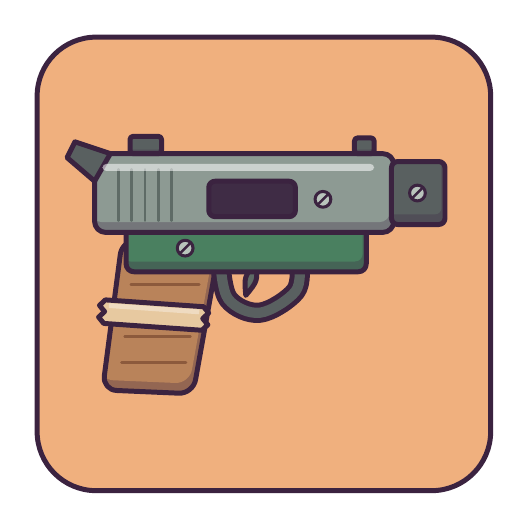
\begin{tikzpicture}
\clip (0,0) rectangle (6,6);
\fill[wallD] [rounded corners=0.75cm] (0.12,0.12) rectangle (5.88,5.88);
\begin{scope}\clip [rounded corners=0.75cm] (0.12,0.12) rectangle (5.88,5.88);
\begin{scope}\clip[rounded corners=0.18cm] (1.2,3.3) -- (2.45,3.3) -- (2.1,1.35) -- (0.95,1.4) -- cycle;
\fill[wood!70!ink,rounded corners=0.18cm] (1.2,3.3) -- (2.45,3.3) -- (2.1,1.35) -- (0.95,1.4) -- cycle;
\fill[wood,rounded corners=0.18cm, shift={(-0.045,0.13)}] (1.2,3.3) -- (2.45,3.3) -- (2.1,1.35) -- (0.95,1.4) -- cycle;
\end{scope}
\draw[inked,rounded corners=0.18cm] (1.2,3.3) -- (2.45,3.3) -- (2.1,1.35) -- (0.95,1.4) -- cycle;
\draw[wooddark, line width=1pt, line cap=round] (1.192,1.75) -- (2.01,1.75);
\draw[wooddark, line width=1pt, line cap=round] (1.232,2.08) -- (2.066,2.08);
\draw[wooddark, line width=1pt, line cap=round] (1.271,2.41) -- (2.122,2.41);
\draw[wooddark, line width=1pt, line cap=round] (1.311,2.74) -- (2.178,2.74);
\filldraw[inked,fill=stone] (0.966,2.244) -- (2.213,2.157) -- (2.288,2.227) -- (2.223,2.306) -- (2.299,2.376) -- (2.234,2.456) -- (0.987,2.543) -- (0.912,2.473) -- (0.977,2.394) -- (0.901,2.324) -- cycle;
\fill[white, opacity=0.35] (1.03,2.44) -- (2.177,2.36) -- (2.181,2.42) -- (1.034,2.5) -- cycle;
\draw[ink, line width=7.299pt, line cap=round, line join=round] plot[smooth, tension=0.6] coordinates {(2.45,3) (2.55,2.55) (2.95,2.38) (3.4,2.65) (3.45,3)};
\draw[metaldark!85!ink, line width=3.699pt, line cap=round, line join=round] plot[smooth, tension=0.6] coordinates {(2.45,3) (2.55,2.55) (2.95,2.38) (3.4,2.65) (3.45,3)};
\filldraw[inked,fill=metaldark] (2.9,3.02) .. controls (2.921,2.783) .. (2.77,2.6) .. controls (2.749,2.837) .. (2.9,3.02) -- cycle;
\begin{scope}\clip[rounded corners=0.1cm] (1.25,2.9) rectangle (4.3,3.5);
\fill[greenE!70!ink,rounded corners=0.1cm] (1.25,2.9) rectangle (4.3,3.5);
\fill[greenE,rounded corners=0.1cm, shift={(-0.045,0.13)}] (1.25,2.9) rectangle (4.3,3.5);
\end{scope}
\draw[inked,rounded corners=0.1cm] (1.25,2.9) rectangle (4.3,3.5);
\begin{scope}\clip[rounded corners=0.14cm] (0.85,3.4) rectangle (4.65,4.4);
\fill[metal!70!ink,rounded corners=0.14cm] (0.85,3.4) rectangle (4.65,4.4);
\fill[metal,rounded corners=0.14cm, shift={(-0.045,0.13)}] (0.85,3.4) rectangle (4.65,4.4);
\end{scope}
\draw[inked,rounded corners=0.14cm] (0.85,3.4) rectangle (4.65,4.4);
\draw[metaldark, line width=1pt, line cap=round] (1.15,3.55) -- (1.15,4.2);
\draw[metaldark, line width=1pt, line cap=round] (1.32,3.55) -- (1.32,4.2);
\draw[metaldark, line width=1pt, line cap=round] (1.49,3.55) -- (1.49,4.2);
\draw[metaldark, line width=1pt, line cap=round] (1.66,3.55) -- (1.66,4.2);
\draw[metaldark, line width=1pt, line cap=round] (1.83,3.55) -- (1.83,4.2);
\filldraw[inked,fill=metaldark!85!ink] (0.85,4.05) -- (0.5,4.35) -- (0.6,4.55) -- (1.05,4.4) -- cycle;
\begin{scope}\clip[rounded corners=0.04cm] (1.3,4.4) rectangle (1.7,4.62);
\fill[metaldark!85!ink!70!ink,rounded corners=0.04cm] (1.3,4.4) rectangle (1.7,4.62);
\fill[metaldark!85!ink,rounded corners=0.04cm, shift={(-0.017,0.05)}] (1.3,4.4) rectangle (1.7,4.62);
\end{scope}
\draw[inked,rounded corners=0.04cm] (1.3,4.4) rectangle (1.7,4.62);
\begin{scope}\clip[rounded corners=0.04cm] (4.15,4.4) rectangle (4.4,4.6);
\fill[metaldark!85!ink!70!ink,rounded corners=0.04cm] (4.15,4.4) rectangle (4.4,4.6);
\fill[metaldark!85!ink,rounded corners=0.04cm, shift={(-0.017,0.05)}] (4.15,4.4) rectangle (4.4,4.6);
\end{scope}
\draw[inked,rounded corners=0.04cm] (4.15,4.4) rectangle (4.4,4.6);
\begin{scope}\clip[rounded corners=0.08cm] (2.3,3.6) rectangle (3.4,4.05);
\fill[ink!88!metaldark!70!ink,rounded corners=0.08cm] (2.3,3.6) rectangle (3.4,4.05);
\fill[ink!88!metaldark,rounded corners=0.08cm, shift={(0,0)}] (2.3,3.6) rectangle (3.4,4.05);
\end{scope}
\draw[inked,rounded corners=0.08cm] (2.3,3.6) rectangle (3.4,4.05);
\fill[white, opacity=0.55, rounded corners=0.05cm] (0.95,4.18) rectangle (4.4,4.27);
\begin{scope}\clip[rounded corners=0.08cm] (4.62,3.5) rectangle (5.3,4.3);
\fill[metaldark!85!ink!70!ink,rounded corners=0.08cm] (4.62,3.5) rectangle (5.3,4.3);
\fill[metaldark!85!ink,rounded corners=0.08cm, shift={(-0.045,0.13)}] (4.62,3.5) rectangle (5.3,4.3);
\end{scope}
\draw[inked,rounded corners=0.08cm] (4.62,3.5) rectangle (5.3,4.3);
\filldraw[inked,fill=metallight,line width=1.1pt] (4.95,3.9) circle (0.1);
\draw[ink, line width=0.9pt, line cap=round] (4.895,3.845) -- (5.005,3.955);
\filldraw[inked,fill=metallight,line width=1.1pt] (3.75,3.82) circle (0.1);
\draw[ink, line width=0.9pt, line cap=round] (3.695,3.765) -- (3.805,3.875);
\filldraw[inked,fill=metallight,line width=1.1pt] (2,3.2) circle (0.1);
\draw[ink, line width=0.9pt, line cap=round] (1.945,3.145) -- (2.055,3.255);
\end{scope}
\draw[inked] [rounded corners=0.75cm] (0.12,0.12) rectangle (5.88,5.88);
\end{tikzpicture}
\end{document}
